\documentclass[letterpaper, 12pt]{article}

\setlength{\topmargin}{0in}
\setlength{\headheight}{0in}
\setlength{\headsep}{0in}
\setlength{\footskip}{0.5in}
\setlength{\textheight}{\paperheight}
\addtolength{\textheight}{-2in}
\addtolength{\textheight}{-\footskip}

\setlength{\oddsidemargin}{0in}
\setlength{\evensidemargin}{0in}
\setlength{\textwidth}{\paperwidth}
\addtolength{\textwidth}{-2in}

\pagestyle{empty}

\usepackage{amsfonts}
\usepackage{polynom}
\usepackage{tikz}

\begin{document}

\begin{center}
\bfseries
San Jos\'{e} State University \\
Fall 2015 \\
Math-8: College Algebra \\
Section 03: MW noon--1:15pm \\
Section 05: MW 4:30--5:45pm \\
\bigskip
Quiz \#11 Solutions)
\end{center}

\bigskip

You may use your book, notes, and homework, but please do not work together or
ask for help from others.

\bigskip

\newcommand{\fillin}{\rule{1.5in}{1pt}}

1. Consider the following graph of a polynomial function, where each grid line
represents 1 unit:

\bigskip

\begin{center}
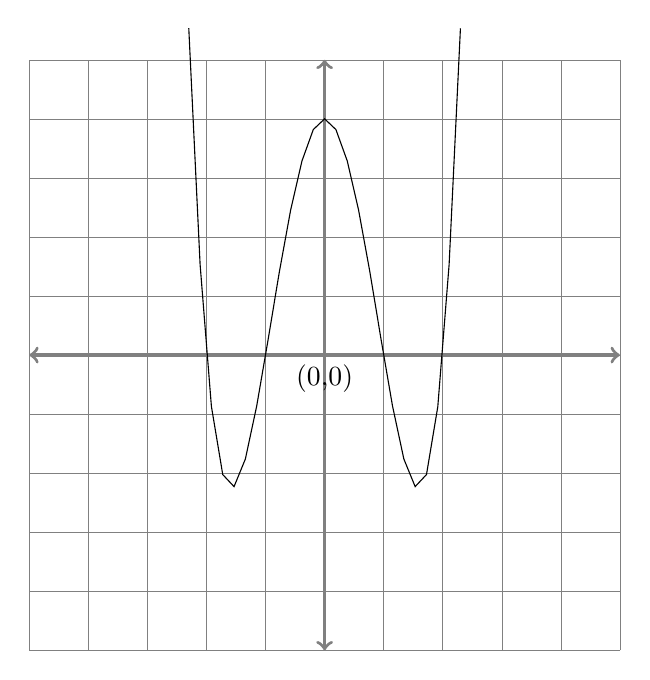
\begin{tikzpicture}[scale=0.75]
\draw [help lines] (-5,-5) grid (5,5);
\draw [help lines, <->, very thick] (-5,0) -- (5,0);
\draw [help lines, <->, very thick] (0,-5) -- (0,5);
\node [below] at (0,0) {(0,0)};
\draw [domain=-2.3:2.3] plot (\x, {(\x)^4-5*(\x)^2+4});
\end{tikzpicture}
\end{center}

\bigskip

What is the remainder when the polynomial is divided by $(x-2)$? Why?

\bigskip

The only important piece of information from this graph is the fact that
$f(2)=0$. This tells us that (2,0) is a zero/x-intercept for $f(x)$, that $x-2$
divides $f(x)$, and thus the remainder is 0.

\bigskip

Some people started with $x^4-5x^2+4$ with no justification why they started
there. At best, they left off the justification or at worst copied this from
someone (cheating). Such efforts received 0 points.

\bigskip

Others started with $f(x)=(x+2)(x+1)(x-1)(x+2)$, which may or may not be true,
but you can't assume a general equation from a sketch, unless the sketch is
something specific like a parabola, circle, or line. Sometimes, people leave
detail out of sketches. But at least this showed that people were thinking
about the intercepts, so partial credit. But then, incredibly, some people
multiplied this out to get $x^4-5x^2+4$. and then divided by $x-2$ to show no
remainder!? But they should have already known this since it is $x-2$ was a
factor in what they started with!!!

2. Without doing the long (or synthetic) division, what is the remainder when
$x^4-2x^3-7x^2+8x+12$ is divided by $(x+2)$? Why?

\bigskip

Just apply the remainder theorem:

\begin{eqnarray*}
f(-2) &=& (-2)^4-2(-2)^3-7(-2)^2+8(-2)+12 \\
      &=& 16+16-28-16+12 \\
      &=& 0 \\
\end{eqnarray*}

Thus, the remainder is 0.

\bigskip

3. Divide $x^2+1$ into $x^5-3x^2+2x-1$. Be sure to express the answer
completely.

\bigskip

When doing the division by hand, be sure to include placeholders for missing
terms.  Thus, the divisor should become $x^2+0x+1$ and the dividend should be
$x^5+0x^4+0x^3-3x^2+2x-1$. Then do the division. Note that the formatting
package that I am using uses blanks instead of the placeholders, so please
pretend that they are there.

\bigskip

\polylongdiv{x^5+0x^4+0x^3-3x^2+2x-1}{x^2+1}

\bigskip

The correct form for the answer here is: $x^3-x-3+\frac{3x+2}{x^2+1}$.

\bigskip

4. Express the answer in (4) per the division algorithm.

\[f(x)=(x^2+1)(x^3-x-3)+(3x+2)\]

5. Sketch the graph of $f(x)=x^4-2x^3-7x^2+8x+12$, showing all $x$ and $y$
intercepts, and behavior as $x\to\pm\infty$. For full credit, show how you
determined the intercepts and behavior, and how you determined the sign of
the function in between the $x$-intercepts.

\bigskip

I was looking for the following steps for full credit:

\begin{enumerate}

\item{Leading coefficient test}

Use this test to determine the behavior of $f(x)$ as $x\to\pm\infty$.
Alternatively, you can use test points below; however, the leading coefficient
test is preferred. In this problem, the degree is even and the leading
coefficient is positive, so the end behavior is like $x^2$.

\item{Determine candidate zeros}

I needed to see why you tried certain candidates. The justification is that you
divide factors of the constant term coefficient by factors of the leading term
coefficient.  Since $a_4=1$ and $a_0=12$, the candidates are:

\[\pm1,\pm2,\pm3,\pm4,\pm6,\pm12\]

Simply starting to use these candidates without justification only received
partial credit.

\item{Find zeros from the candidates}

Just plug the candidates into $f(x)$. By the remainder theorem, actual zeros
will have $f(k)=0$, meaning $f(x)$ is divisible by $x-k$. There is no need
to do long or synthetic division here to determine if a candidate is actually
a zero.

\item{Divide out candidates}

Once a candidate is identified by $f(k)=0$ then $x-k$ should be divided out
from $f(x)$ so that we get $f(x)=(x-k)g(x)$. The process should then be
repeated recursively with $g(x)$ to find additional factors. Note that some
people found all the factors first, without dividing out found ones
immediately. This is OK; however, it is more work and it will miss repeated
zeros - e.g., if $f(x)$ can be divided by $(x-1)^2$. If you use this method,
you must keep dividing by a found zero until it no longer divides. I can
pretty much guarantee that a question on the exam will have such repeated
zeros - so beware!

\bigskip

So here is how I proceeded to solve this problem.

\begin{eqnarray*}
f(1) &=& 1-2-7+8+12\ne0 \\
f(-1) &=& 1+2-7-8+12=0 \\
\end{eqnarray*}

So $x+1$ divides $f(x)$. Doing the division:

\bigskip

\polylongdiv{x^4-2x^3-7x^2+8x+12}{x+1}

\bigskip

So, $f(x)=(x+1)g(x)=(x+1)(x^3-3x^2-4x+12)$. We now continue the process with
$g(x)$ to pull out more factors. Once again, $a_n=1$ and $a_0=12$, so we have
the same candidates. If $x=1$ did not work before, then it certainly won't work
now, so we don't need to consider it again; however, $x=-1$ might be a repeated
root, so we need to try it again:

\[g(-1)=-1-3+4+12\ne0\]

So $x=-1$ is not repeated. Continuing:

\[g(2)=8-12-8+12=0\]

So we need to divide out $x-2$:

\bigskip

\polylongdiv{x^3-3x^2-4x+12}{x-2}

\bigskip

and now $f(x)=(x+1)(x-2)(x^2-x-6)$. We could continue in this fashion; however,
we know how to finish the factoring:

\[f(x)=(x+1)(x-2)(x-3)(x+2)\]

We now have our x-intercepts for the graph.

\item{Find the y-intercept}

\[f(0)=0-0-0+0+12=12\]

\item{Use test points to determine sign in intervals between x-intercepts}

\begin{tabular}{c|cccc|c}
 & $(x+1)$ & $(x+2)$ & $(x-2)$ & $(x-3)$ & \\
\hline
-1.5 & $-$ & $+$ & $-$ & $-$ & $-$ \\
0 & $+$ & $+$ & $-$ & $-$ & $+$ \\
2.5 & $+$ & $+$ & $+$ & $-$ & $-$ \\
\end{tabular}

\bigskip

Alternatively, some people use the multiplicity of a factor to determine whether
or not the graph passes through the zero to change sign: factors with odd
exponents do and factors with even exponents do not.

\item{Sketch the graph, labeling all intercepts}

\begin{center}
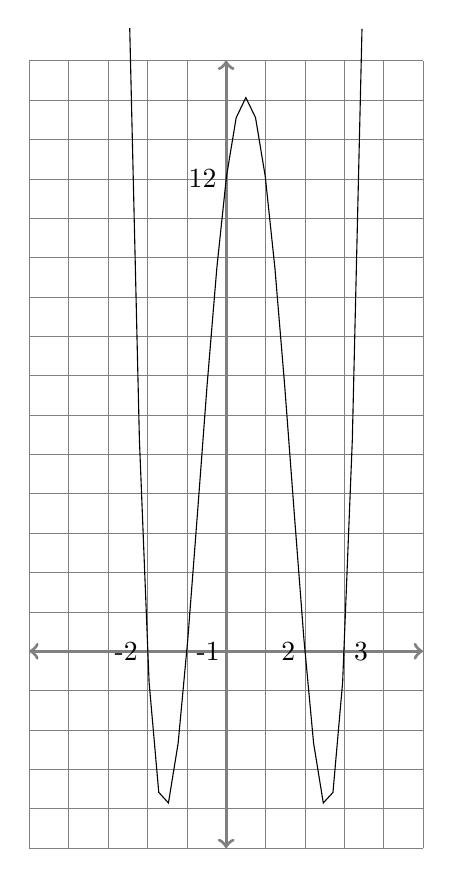
\begin{tikzpicture}[scale=0.5]
\draw [help lines] (-5,-5) grid (5,15);
\draw [help lines, <->, very thick] (-5,0) -- (5,0);
\draw [help lines, <->, very thick] (0,-5) -- (0,15);
\node [left] at (-2,0) {-2};
\node [right] at (-1,0) {-1};
\node [left] at (2,0) {2};
\node [right] at (3,0) {3};
\node [left] at (0,12) {12};
\draw [domain=-2.45:3.45] plot (\x, {(\x)^4-2*(\x)^3-7*(\x)^2+8*(\x)+12});
\end{tikzpicture}
\end{center}

\end{enumerate}

\end{document}
